\begin{frame}{Robot Model}{}
  \begin{columns}[T] % align columns
    \begin{column}{.55\textwidth}
      \begin{itemize}
      \item Differential drive robots
      \item Each robot has a unique \textbf{ID}
      %\item Use a vector $p = [x, y,
       % \theta]^T$ to represent robot's \textbf{pose}
      \item Each robot has a \textbf{range} within which it can
        sense and communicate with other robots
      \item Each robot gets \textbf{observation} of its neighbors'
        IDs and relative poses in its body frame
      \end{itemize}
    \end{column}%
    % right column
    \begin{column}{.45\textwidth}
        \begin{figure}
    \centering
    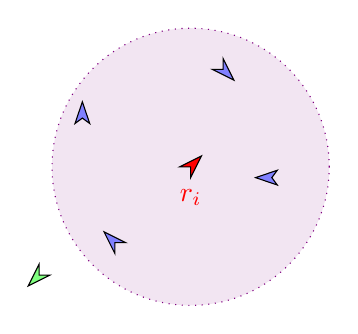
\begin{tikzpicture}[scale=0.55]
        \draw[dotted, violet, fill=violet!10] (3, 3) circle (3.2);
        \draw[fill=red] (3,3) -- (2.75,3) -- (3.25,3.25) -- (3,2.75) -- cycle;
        \node[color=red] at (3, 2.3) {$r_i$};           
        \draw[fill=blue!50] (0.5,4.5) -- (0.33,4) -- (0.5,4.125) -- (0.67,4)-- cycle;
        \draw[fill=blue!50] (4,5) -- (3.75,5.5) -- (3.75,5.25) -- (3.5,5.25)-- cycle;
        \draw[fill=blue!50] (1,1.5) -- (1.25,1) -- (1.25,1.25) -- (1.5,1.25)-- cycle;
        \draw[fill=blue!50] (5,2.92) -- (4.5,2.75) -- (5,2.58) -- (4.875,2.75)-- cycle;
        \draw[fill=green!50] (-0.5,0.5) -- (-0.5,0.75) -- (-0.75,0.25) -- (-0.25,0.5) -- cycle;
    \end{tikzpicture}
\end{figure}
\begin{center}
    Robot $r_i$ has 4 neighbors
\end{center}
    \end{column}%
  \end{columns}
\end{frame}